\chapter{Results}
\label{chapter3}

\section{Running Xv6 with the solution}
A Dockerfile is provided with the project to ensure a consistent compilation
and execution environment for development (see Appendix \ref{appendix:c:1}).
The file contains instructions for Docker to build a container with the tools
required to compile and run Xv6 in QEMU.

Running the solution is simple, create a container from the provided Dockerfile,
mount the project directory and run `\mintinline{bash}{make qemu}'. Port 5900 may
need to be forwarded from the container to access the VNC output. A configuration
for Visual Studio Code also exists in the project, so loading the project and
pressing the F5 key should also run the project.

Once QEMU is running, connect a VNC client to localhost:5900 to view the display
output.

\section{Boot sequence test}

When the project boots, we should see two things:
\begin{itemize}
    \item Boot image, one for each CPU in the system (figure \ref{figure:bootimg})
    \item The window borders once the window manager finishes initialisation (figure \ref{figure:winborder})
\end{itemize}

\begin{figure}[H]
    \centering
    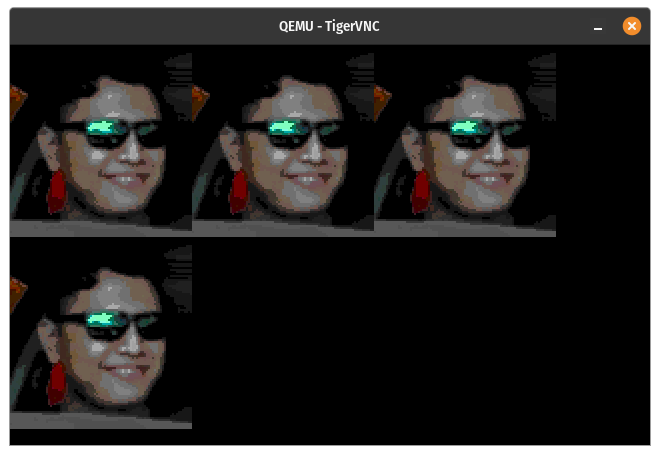
\includegraphics[width=8cm]{bootimage.png}
    \caption{Boot image test}
    \label{figure:bootimg}
\end{figure}

\begin{figure}[H]
    \centering
    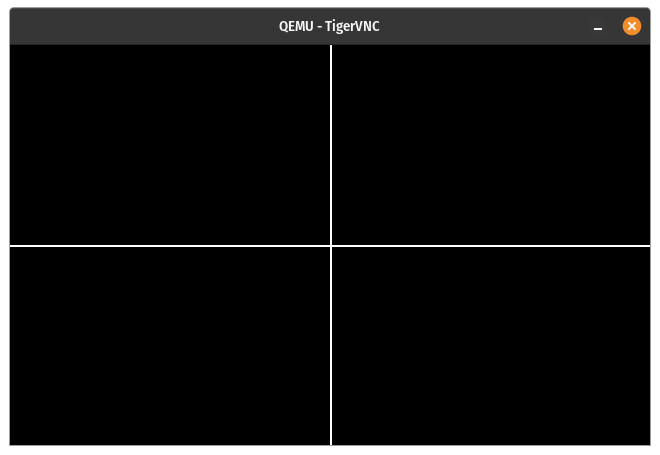
\includegraphics[width=8cm]{active0.png}
    \caption{Window border drawing test}
    \label{figure:winborder}
\end{figure}

We can see the boot image works as expected, repeated 4 times offset properly
for each CPU core being initialised. The window borders are also being drawn
once the system finishes booting.  

\section{Window switching}

When pressing the control character specified earlier, we should see the active
window being cycled (the red border indicating the active window) and then back to no
active window (figure \ref{figure:windowswitch}). 

\begin{figure}[H]
    \centering
    \begin{tabular}{cc}
    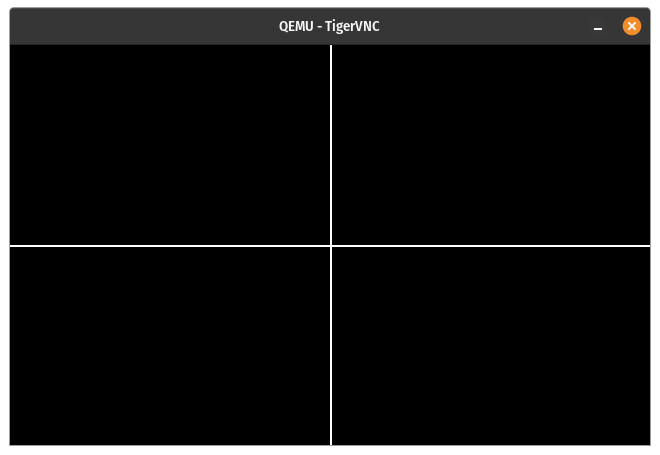
\includegraphics[width=4cm]{active0.png} & 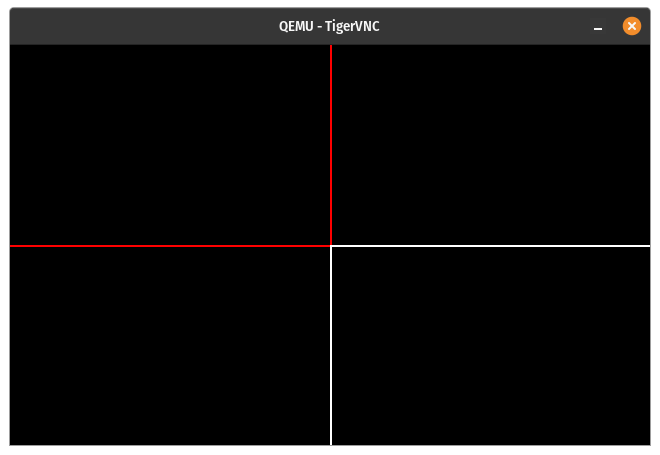
\includegraphics[width=4cm]{active1.png} \\
    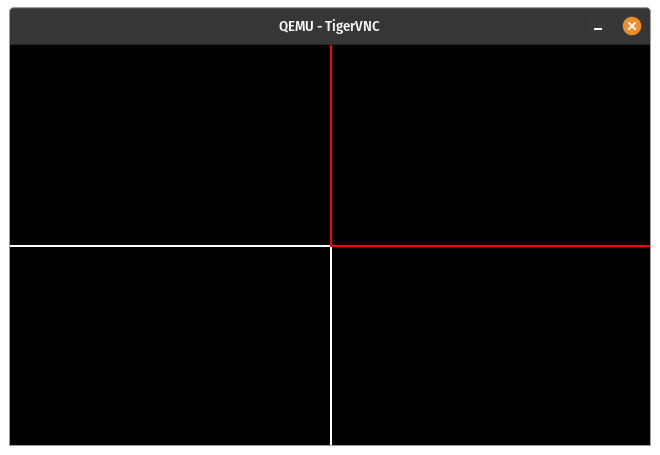
\includegraphics[width=4cm]{active2.png} & 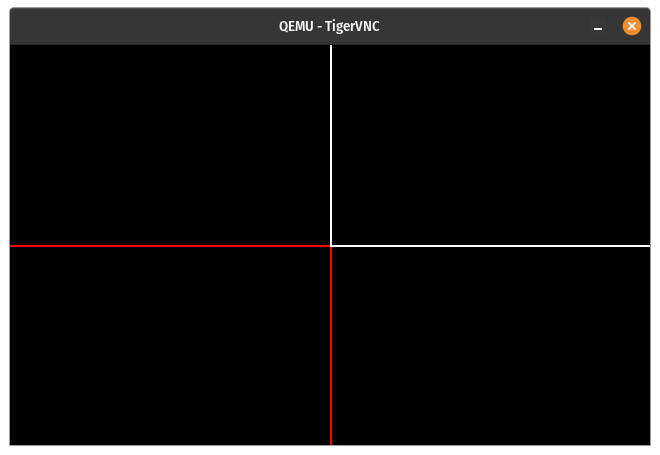
\includegraphics[width=4cm]{active3.png} \\
    \end{tabular}
    \caption{Active window cycling test}
    \label{figure:windowswitch}
\end{figure}

\section{Simple display and input test program}

Using the graphics library written in Chapter \ref{chapter2:impl:usrlib}, we can
write a simple program to test the event queue and basic drawing.

\begin{listing}[H]
    \begin{minted}{c}
    // open the first available window
    window_handle win = window_create();

    // go through the palette
    uint8 cc = 0;
    struct windowevent evt;
    struct window_dim dim = window_getdimensions(win);
    printf("%d x %d\n", dim.width, dim.height);
    while (1)
    {
        if (window_pollevent(win, &evt, 1) == 1)
        {
            if (evt.payload == 113) // q was inputted
                break;
            cc = cc + 1 % 0xFF;
            window_drawchar(win, 0, 0, ' ', 0x00);
            window_drawchar(win, 0, 0, evt.payload, cc);
            window_drawrect(win, 0, 16, dim.width, dim.height, cc);
        }
    }
    window_destroy(win);
    exit(0);
    \end{minted}
\end{listing}

This program draws the character from the event queue and cycles through the colour palette
It uses the graphics library to allocate a window, poll the event queue, and draw
characters and rectangles to the window.

\begin{figure}[H]
    \centering
    \begin{tabular}{cc}
    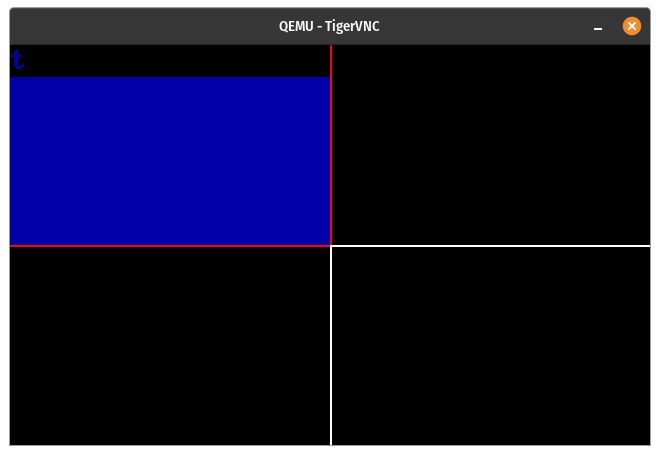
\includegraphics[width=5cm]{windowtest0.png} & 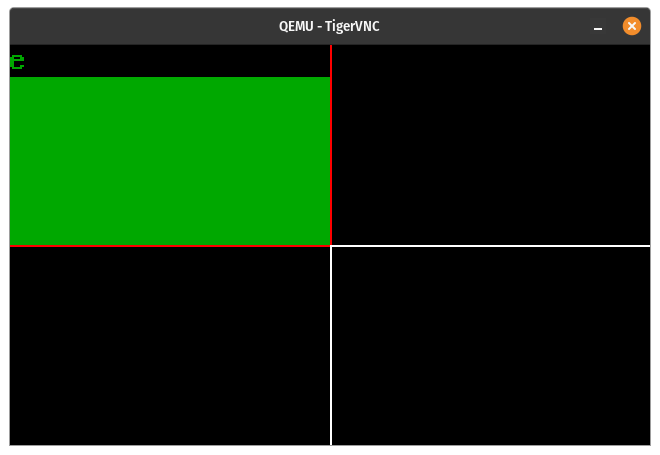
\includegraphics[width=5cm]{windowtest1.png} \\
    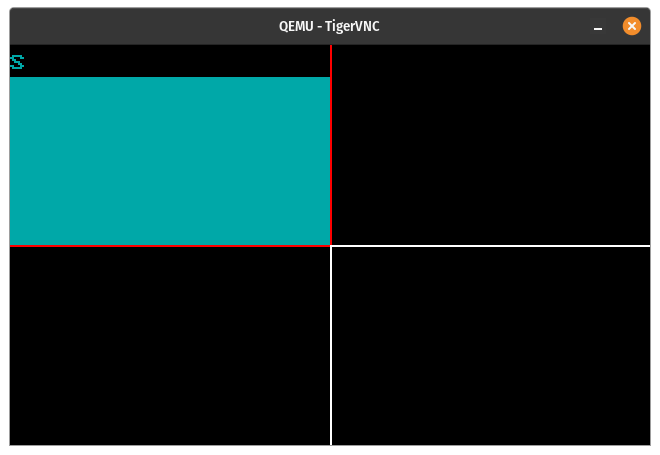
\includegraphics[width=5cm]{windowtest2.png} & 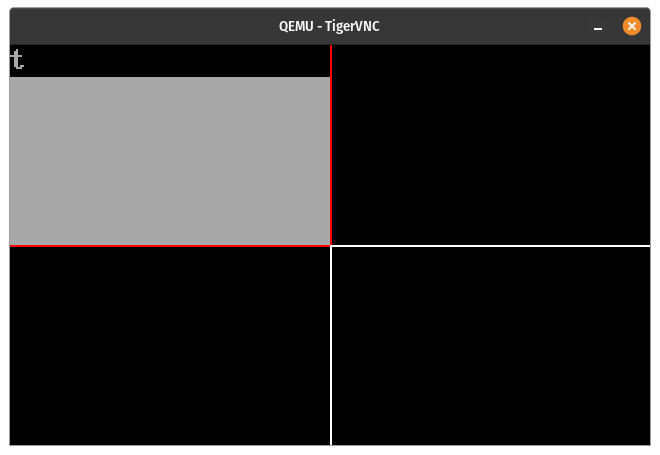
\includegraphics[width=5cm]{windowtest3.png} \\
    \end{tabular}
    \caption{user/windowtest program}
    \label{figure:windowtest}
\end{figure}

The screenshots in figure \ref{figure:windowtest} show that the window is
properly receiving input events and that the 256 color palette has been loaded.

\section{High framerate test}

We will test the implementation by writing a simple game that clears the screen
and draws game sprites multiple times a second (see Appendix \ref{appendix:c:9} for code).

\begin{figure}[H]
    \centering
    \begin{tabular}{cc}
    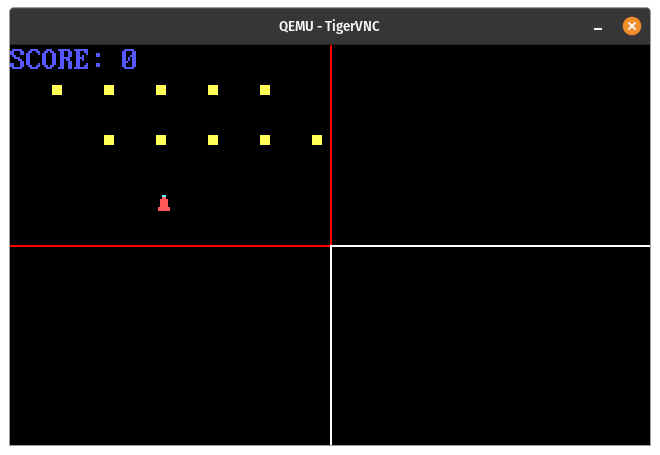
\includegraphics[width=5cm]{game0.png} & 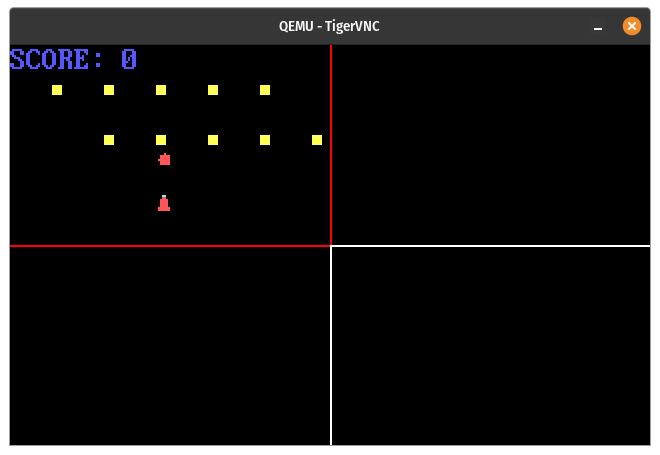
\includegraphics[width=5cm]{game1.png} \\
    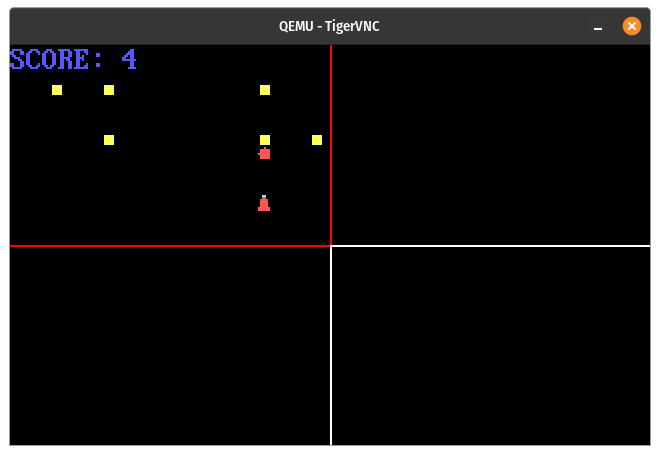
\includegraphics[width=5cm]{game2.png} & 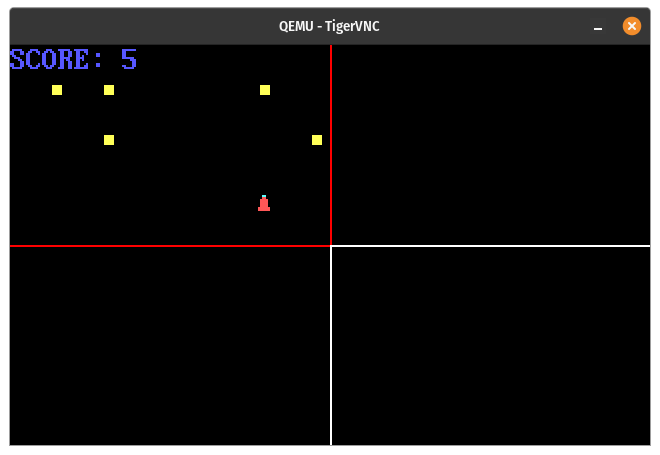
\includegraphics[width=5cm]{game3.png} \\
    \end{tabular}
    \caption{user/game program}
    \label{figure:game}
\end{figure}

While running the program, there is a noticeable flickering, and input delay.
This is to be expected as our graphics is currently single buffered, so the display
will also show the cleared screen between frames. The input delay is probably caused
by the numerous system calls when drawing each object to the screen. The game text
and the bullets also use \mintinline{c}{window_drawchar()}
and \mintinline{c}{window_drawcircle()}, which has a slow implementation in which two system calls are
made per pixel drawn.

Most if not all of these issues can be resolved by implementing software side
double buffering. The graphics library or the kernel will need to store the
current frame being written to in memory, and copy it to the main VGA
framebuffer when it is ready for display. This will most likely eliminate
flickering, and if the buffering is done in userspace, will reduce input lag as
the amount of system calls per frame would be reduced to only one.